\subsection{Traffic investigation}
This section describes the traffic analysis done on the RF layer and the HCI layer. The third section describes how the data found at the two layer have been tried to be correlated.
\subsubsection{RF layer}
\label{subsubsection:rflayer}
Regarding the RF layer a few messages can be seen there. Most of the packets seen are the NULL and POLL messages, these are keep alive messages. During the captures the Ubertooth is only looking at channel 0 on which these packets are sent.
But there are also some other packets that are decoded by the Ubertooth. These packets over the RF layer are of a different types. The packet decoded are of type DV/3-DH1, AUX1, AFH, DM1, HV1, DH5/3-DH5. An explanation of these packet types are explained in this appendix \ref{app:types}.

The only valuable information that could be output from this data analysis is that the packets sent between the smartwatch and the phone are fragmented as they contain different LLID parameters (which specifies if the payload is the start or the continuation of a L2CAP or LMP message). The packets their payload is encrypted.

\subsubsection{HCI layer}
From the HCI captures, some conclusions can be drawn. Indeed, during the pairing process, some parameters are negotiated regarding the future communication between the two devices. SSP introduces IO capabilities that permits to exchanged what would be the pairing model based on the capability of the master and slave device. 
\begin{figure}[!h]
	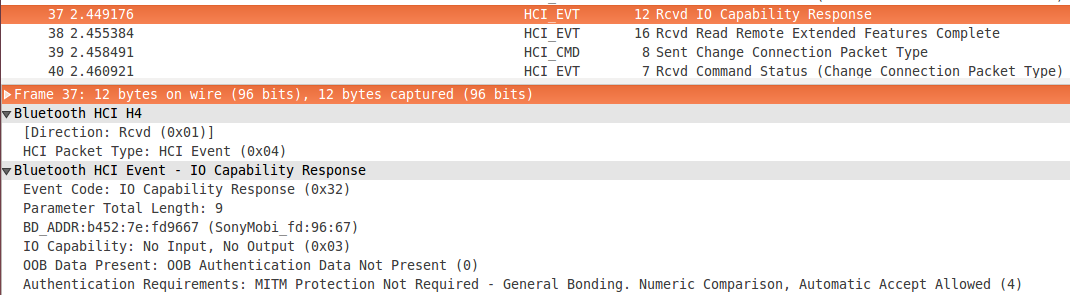
\includegraphics[width=270px]{images/IO_PARAM.png}
	\caption{IO capabilities found during the pairing process at the HCI layer}
	 \label{fig:io1}
\end{figure}
The pairing process analysis shows that is based on JustWork mechanism. Indeed, as shown in \ref{fig:io1} the Smartwatch claim not to have any input or output and that it does not have OOB authentication. Then the two devices agree to set up their connection with the JustWork mechanism that involves automatic accept of the numeric comparison. This mechanism is not protected from a MiTM attack \cite{MiTMjustworks}.

Then the LMP parameters are exchanged (see figure 7 below) to choose the LMP parameters that will be used during this communication. 
\begin{figure}[!h]
  \begin{center}
	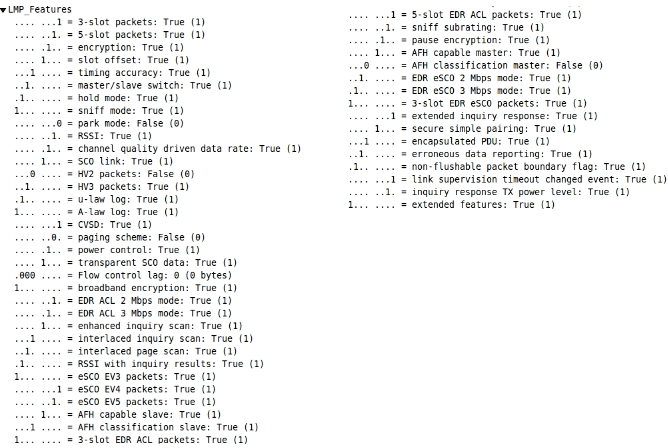
\includegraphics[width=350px]{images/LMP_PARAM.jpg}
	\label{fig:lmp}
	\caption{LMP Parameters found during the pairing process at the HCI layer}
  \end{center}
\end{figure}

From there, it is true to say that the communication uses SSP and is encrypted and encapsulated. It is even possible to retrieve the link keys used for encryption at this level. The link keys are always updated after a new pairing.
\newpage
\subsubsection{Correlation of the two layers}

%Why cant we correlate the packet seen on Rf to hci? 
%Maybe we should trey to decrypt a packet using the key we found nat the hci. Just to proove that it is possible to decrypt the packets if we would have the key. ANd we would have the key maybe if the ubertooth was doing what we did.
First thing to notice is that the POLL and NULL packet are not available at the HCI layer. These are destined and processed at the link controller layer so they cannot be seen. With this said these packets will be seen during the correlation between what is seen on the Ubertooth and in the HCI. More interesting are the other packages mentioned in section \ref{subsubsection:rflayer}. These packets can be seen every so often and they come in a wide variety of packet types and have different payloads and sizes.
These are the packets that can be found and unwhitened by the Ubertooth.
Some examples are seen in appendix \ref{app:roguepackets}. These are all the 3-DH1 packets from one experiment. Looking at the first packet in appendix \ref{app:roguepackets} there are a few things that can be seen. The first line of the output seen in the appendix contains information about the packet when and how it was found. This is primarily debug information. The most important part of this first line is this:
The \textbf{ch}, this is the channel in which the packet was found.
The \textbf{LAP}, which is the sender's lower address part. \pend
An unwhitened packet is divided in a few fields. Type, LT\_ADDR, flow, payload length and data.
The first value is the \textbf{type}. The reason that the type has two values is that for different data rates the packet type can differ. So in this example it could be a DV or a 3-DH1 packet. The SW2 has no voice capabilities and knows high data transfer rate. This means it is very likely that the latter of the two is the packet type. This is enforced the specifications \cite{bt3.0}(page 308).
Next is the \textbf{LT\_ADDR} this used to determine which is used by each receiving device to determine if the packet addressed to them, but it is also used for internal routing.
The \textbf{LLID} is the (Logical Link Identifier). This is used to give information about the packet. For example if the value is $2$ this means that this is the start of the packet or it is standalone. It can also indicate that it is control information between the link manager of the master and the slave. This is indicated by a LLID of $3$.
The value the \textbf{flow} is used to control the flow per logical link. This can be $1$ for go or $0$ for stop. This means that for all the shown packets that the transmission should be stopped first before sending more packets.
For more detailed information of these fields look in the specifications that can be found here \cite{bt3.0}.
After seeing the Bluetooth specifications it is no surprise that these packets cannot be seen on the HCI layer. These packets are used for the control of the data packages and other control information between master and and slave. These packets are not relevant for the higher layers and cannot be seen. We do not know what and why it controls. This means that the information gotten from the Ubertooth cannot be correlated to the information that is seen on the HCI layer. The experiment did not help make sense of the data seen.